\documentclass[a4paper, 11pt]{article}

\usepackage[swedish]{babel}
\usepackage[utf8]{inputenc}
\usepackage[T1]{fontenc}
\usepackage{lmodern}

\usepackage{tikz}

\tikzset{
  excl/.style = {circle, draw=black, inner sep=0pt, minimum size=4pt}
}

\tikzset{
  incl/.style = {circle, draw=black, fill=black, inner sep=0pt, minimum size=4pt}
}


\usepackage{pgfplots}


\usepackage{graphicx}
\usepackage{caption}
\usepackage{subcaption}

\usepackage{enumitem}

\usepackage{multicol}

\usepackage{amsmath}
\usepackage{amsfonts}

\begin{document}

\title{
    \textbf{MM2001: Inlämning 4}
}
\author{Johan Montelius}
\date{HT 2026}

\maketitle

\section*{(i)}
{\em Betrakta en godtycklig fyrhörning med hörnen A, B, C, D och
  använd beteckningen $f_1 = \overrightarrow{DA}$ och $f_2 =
  \overrightarrow{DC}$ . Punkten P delar sträckan AB i förhållandet 2 : 1
  och punkten Q delar sträckan BC i förhållandet 1 : 2. Vektorn $\vec{w}$
  pekar från punkten punkten P till punkten Q.

\begin{enumerate}[label=(\alph*)]
\item Ge en skiss, som innehåller alla ovannämnda punkter och vektorer.
\item Uttryck $\overrightarrow{AC}$ som en linjärkombination av $f_1$ och $f_2$.
\item Uttryck $w$ som en linjärkombination av $f_1$ och $f_2$.
\end{enumerate}
}

\subsection*{a)}

\begin{center}
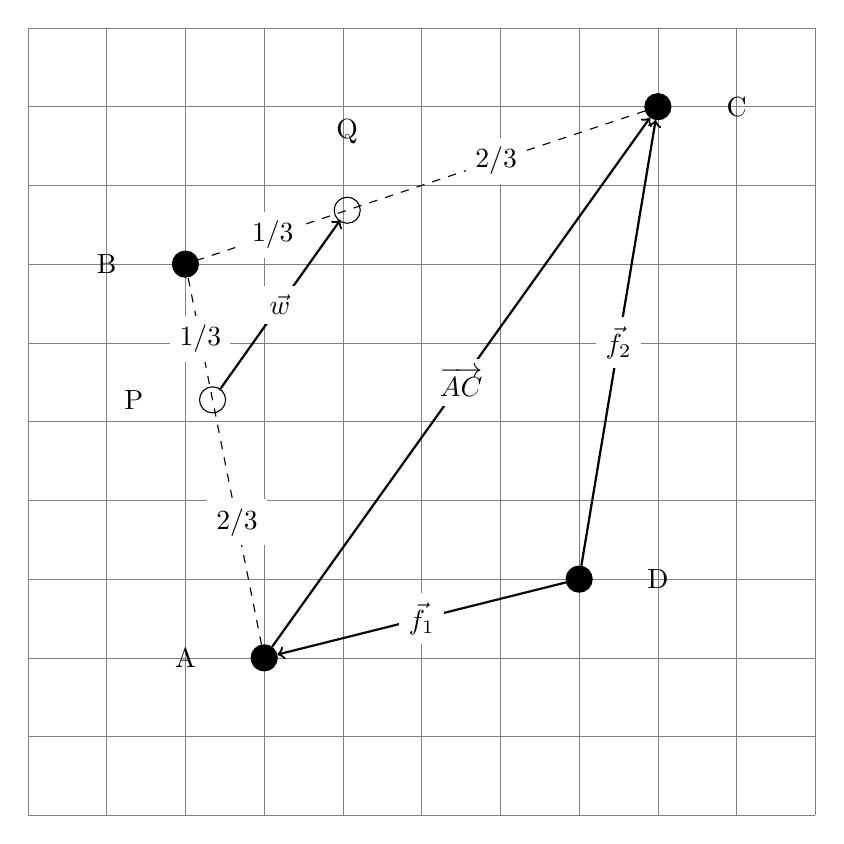
\begin{tikzpicture}
\draw[step=1cm,gray,very thin] (0,0) grid (10,10);

\node[draw, fill, circle] (a) at (3,2) {};
\node[draw, fill, circle] (b) at (2,7) {};
\node[draw, fill, circle] (c) at (8,9) {};
\node[draw, fill, circle] (d) at (7,3) {};
\node[left of = a] {A};
\node[left of = b] {B};
\node[right of = c] {C};
\node[right of = d] {D};

\draw[->, thick] (d) -- (a) node[midway, fill=white] {$\vec{f_1}$};
\draw[->, thick] (d) -- (c) node[midway, fill=white] {$\vec{f_2}$};

\draw[dashed] (a) -- (b) node[pos=2/6, fill=white] {2/3} node[pos=2/3] (p) {} node[pos=5/6,fill=white] {1/3};
\draw[dashed] (c) -- (b) node[pos=2/6, fill=white] {2/3} node[pos=2/3] (q) {} node[pos=5/6,fill=white] {1/3};

\node[draw, circle] at (p) {};
\node[draw, circle] at (q) {};

\node[left of = p] {P};
\node[above of =  q] {Q};


\draw[->, thick] (a) -- (c) node[midway, fill=white] {$\overrightarrow{AC}$};
\draw[->, thick] (p) -- (q) node[midway, fill=white] {$\vec{w}$};



\end{tikzpicture}
\end{center}

\subsection*{b)}

Vektorn $\overrightarrow{AC}$ kan uttryckas som: $$f_2 - f_1$$.

Detta eftersom:
\begin{align}
  \overrightarrow{AC} &= C - A \\
  &= C - D - A + D \\
  &= (C -D) - (A - D)\\
  &= \overrightarrow{DC} - \overrightarrow{DA}\\
  &= f_2 - f_1
\end{align}


\subsection*{c)}

Vektorn $w$ kan uttryckas som: $$1/3 (f_2 - f_1)$$.

Detta eftersom:
\begin{align}
  \overrightarrow{PQ} &= (P - Q) \\
  &= (A + 2/3 \overrightarrow{AB}) - (C + 2/3 \overrightarrow{CB}) \\
  &= (A + 2/3 (B - A)) - (C + 2/3 (B - C)) \\
  &= (A + 2/3 B - 2/3 A) - (C + 2/3 B - 2/3 C) \\
  &= A + 2/3 B - 2/3 A - C - 2/3 B + 2/3 C \\  
  &= A - 2/3 A - C + 2/3C \\
  &= 1/3 A - 1/3 C\\
  &= 1/3 \overrightarrow{AC}\\
  &= 1/3 (f_2 - f_1) \; \text{från uppgift b)}\\ 
\end{align}



\section*{(ii)}

{\em Antag att vi har 3 stycken vektorer, $\vec{v_1}$, $\vec{v_2}$, och $\vec{v_3}$ i $\mathbb{R}_3$.




\begin{enumerate}[label=(\alph*)]
  \item Vad är definitionen av en linjärkombination av dessa vektorer?

  \item Betrakta alla vektorer som är en linjärkombination av $v_1$ och
    $v_2$. Beskriv denna mängd geometriskt med ord (dvs inte bara som en
    formel).
\end{enumerate}
}


\subsection*{a)}

En {\em linjärkombination}, $\vec{l}$, av de tre vektorerna är en vektor som kan skrivas som en summa av de tre, godtyckligt skalade, vektorerna. Vi har har:
$$ \vec{l} = s_1\times\vec{v_1} + s_2\times\vec{v_2} + s_2\times\vec{v_3}  \;\; \text{där}\; s_1,s_2,s_3 \in \mathbb{R}.$$

\subsection*{b)}

Givet att $\vec{v_1}$ och $\vec{v_2}$ är linjärt oberoende så kommer
mängden av linjärkombinationer av $\vec{v_1}$ och $\vec{v_2}$ beskriva
ett plan i $\mathbb{R}_3$. Är vektorerna linjärt beroende men båda skilda
från nollvektorn så får vi en linje. Är båda vektorerna lika med
nollvektorn får vi endast nollvektorn. 




\section*{(iii)}

{\em Uttryck nollvektorn $\overrightarrow{0}$ som en icke-trivial linjärkombination av vektorer i frågan ovan.
Du får gärna göra skissen per hand och lämna in som pdf tillsammans med din annars
datorskrivna lösning.}

Skall vi ha en {\em icke-trivial} linjärkombination så kräver det att
vektorerna inte är linjärt oberoende. Är vektorerna linjärt oberoende
så finns endast den triviala lösningen där vi sätter all parametrar
till noll.

Att vi har tre linjärt beroende vektorer i $\mathbb{R}_3$ betyder att
de ligger i samma plan. För att göra det lite intressant kan vi anta
att vektorerna är parvis linjärt oberoende av varandra (vi har
inte två vektorer som är parallella). 


Eftersom vi endast rör oss i ett plan kan vi rita upp det planet i en
2D-graf för att göra det enklare att illustrera. Nedanstående graf
visar hur tre linjärt beroende vektorer kan ha en icke-trivialt uttryck
för nollvektorn:$$ \overrightarrow{0} = v_1 + 4 v_2 + 7 \vec{v_3}.$$



\begin{center}
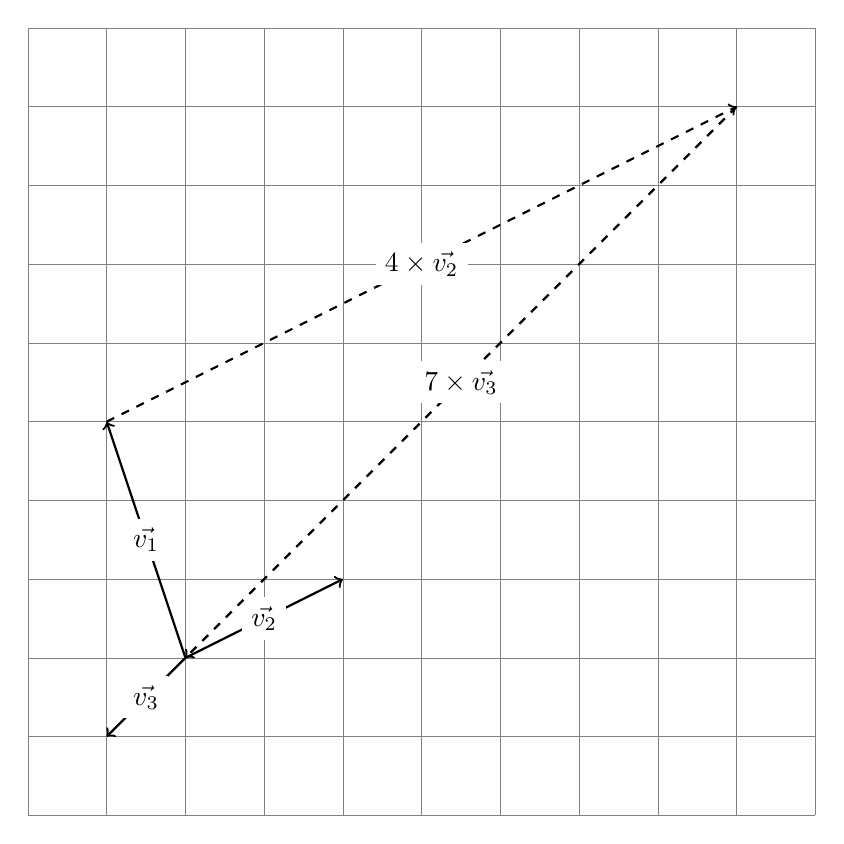
\begin{tikzpicture}
\draw[step=1cm,gray,very thin] (-2,-2) grid (8,8);

\coordinate (v1) at (-1,3);
\coordinate (v2) at (2,1);
\coordinate (v3) at (-1,-1);

\coordinate (v12) at (7,7);

\draw[->, thick] (0,0) -- (v1) node[midway, fill=white] {$\vec{v_1}$};
\draw[->, thick] (0,0) -- (v2) node[midway, fill=white] {$\vec{v_2}$};
\draw[->, thick] (0,0) -- (v3) node[midway, fill=white] {$\vec{v_3}$};

\draw[->, dashed, thick] (v1) -- (v12) node[midway, fill=white] {$4 \times \vec{v_2}$};
\draw[->, dashed, thick] (v12) -- (0,0) node[midway, fill=white] {$7 \times \vec{v_3}$};






\end{tikzpicture}
\end{center}






\end{document}


